\section{Dataset and Audit}
\label{sec:dataset}

Three public, MIT-licensed sources supply real diagrams, point coordinates and human marks. Geometry3K \cite{lu2021intergps} has \nGeometryProblems{} problems with logic-form annotations and point positions; PGDP5K \cite{zhang2022pgdp} has \nPgdpDiagrams{} diagrams with pixel-accurate primitives and marks read from printed symbols; PGPS9K \cite{zhang2023pgps} has \nPgpsDiagrams{}.

\paragraph{The published split leaks.} Only \nGeometryFigures{} distinct figures underlie the \nGeometryProblems{} problems, and because the published split cuts by problem, \pctGeometryTestShareFigure\% of test images have a twin in training or validation. We clustered duplicates across all three and re-split Geometry3K by figure into \nFiguresTrain{} / \nFiguresVal{} / \nFiguresTest{} figures. The \nHeldoutFigures{} test figures of PGDP5K that Geometry3K never reproduced are an unseen source; \nPoolFigures{} PGPS9K figures outside every test set are the unlabelled pool. PGDP5K's cleaner annotation is used wherever it exists.

\paragraph{The marks leave most true relations unmarked.} Over the curated Geometry3K figures the verifier of Section~\ref{sec:verifier} finds that \pctUnmarkedGParallel\% of the parallel pairs in the drawings carry no mark, as do \pctUnmarkedGPerpendicular\% of the perpendicular pairs and every one of the \nUnmarkedGTangent{} tangencies. The marks are seldom wrong (on the held-out source \nAssOnlyHo{} fail the ruler against \nGeomOnlyHo{} unmarked true ones), only incomplete: a textbook marks what the problem needs. Every query therefore carries two label vectors, \emph{asserted} and \emph{geometric}, and the geometric one is the headline.

\paragraph{The witnesses side by side.} The fine-tuned model of Section~\ref{sec:results} scores \fFtId{} and \fFtHo{} macro-F1 against geometric labels on the real test sets and \fFtIdAss{} and \fFtHoAss{} against the marks. The gap is the labels: where the drawing says yes and the mark says nothing, the model says yes \posRateGeomOnlyHo\% of the time, so \shareAssErrorsLabelsHo\% of its ``errors'' against the marks are decisions where it sides with the ruler. Yet \shareGeomErrorsMarkHo\% of its errors against the ruler are cases where it sided with the mark, mostly tick bars asserting an equality the drawing does not keep (Fig.~\ref{fig:audit}).

\begin{figure}[tbp]
  \centering
  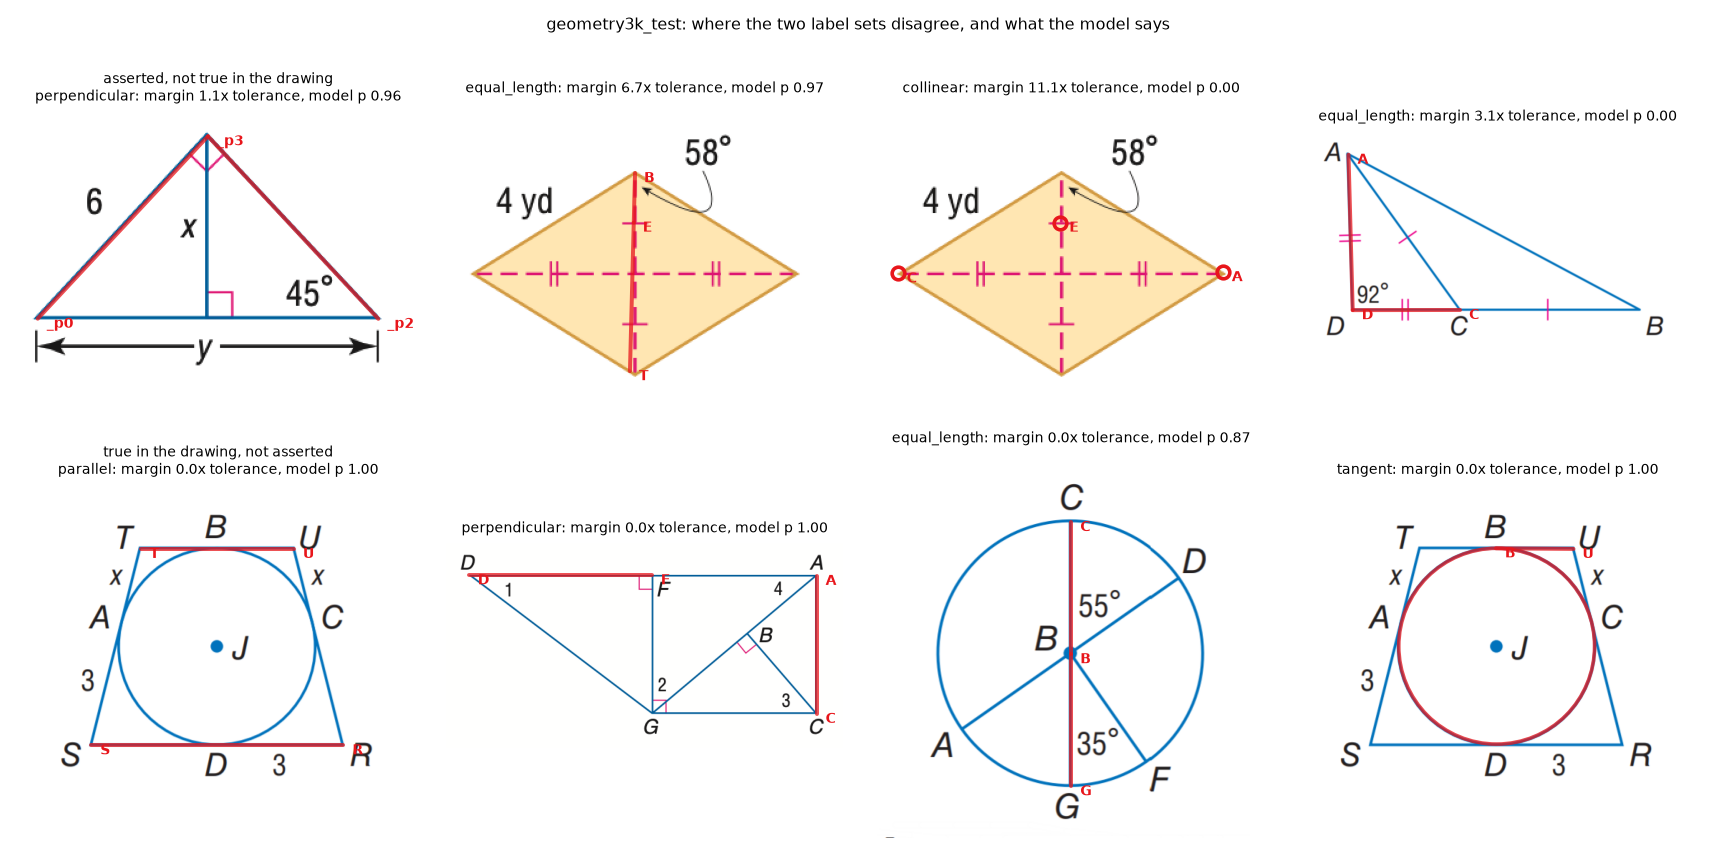
\includegraphics[width=\textwidth]{audit_examples_model}
  \caption{Marked relations the drawing breaks (top) and unmarked ones it keeps (bottom), with the model's answer.}
  \label{fig:audit}
\end{figure}
